\begin{table*}[t]
\caption{Held-out test results for the CNN experiments. Values are reported as mean $\pm$ standard deviation across five folds. Bold values indicate the highest mean balanced accuracy within each experiment.}
\label{tab:cnn-experiment-results}
\centering
\small
\begin{tabular}{@{}lrrrr@{}}
\toprule
Model & BCC (\%) & Recall (\%) & Precision (\%) & Macro F1 (\%) \\
\midrule
\multicolumn{5}{c}{\textbf{Experiment from Maia et al. \citep{MAIA2024122418}}} \\
\midrule
ResNet-50 & $91.38 \pm 1.18$ & $91.77 \pm 0.72$ & $91.77 \pm 0.72$ & $91.77 \pm 0.72$ \\
MobileNet & $91.49 \pm 0.77$ & $91.57 \pm 0.61$ & $91.57 \pm 0.61$ & $91.57 \pm 0.61$ \\
DenseNet-121 & $\mathbf{91.91 \pm 0.84}$ & $91.93 \pm 0.75$ & $91.93 \pm 0.75$ & $91.93 \pm 0.75$ \\
\midrule
\multicolumn{5}{c}{\textbf{Experiment 1: Original-comparable split}} \\
\midrule
MobileNetV2 & $90.57 \pm 0.52$ & $90.57 \pm 0.52$ & $88.46 \pm 1.10$ & $89.37 \pm 0.81$ \\
DenseNet-121 & $\mathbf{91.72 \pm 0.50}$ & $91.72 \pm 0.50$ & $90.16 \pm 0.43$ & $90.87 \pm 0.40$ \\
ResNet-50 & $89.86 \pm 1.12$ & $89.86 \pm 1.12$ & $88.32 \pm 0.98$ & $88.98 \pm 0.95$ \\
\midrule
\multicolumn{5}{c}{\textbf{Experiment 2: Patient-first grouped split}} \\
\midrule
MobileNetV2 & $57.07 \pm 1.57$ & $57.07 \pm 1.57$ & $55.56 \pm 3.66$ & $54.99 \pm 3.49$ \\
DenseNet-121 & $\mathbf{59.41 \pm 3.18}$ & $59.41 \pm 3.18$ & $59.12 \pm 4.30$ & $57.64 \pm 2.82$ \\
ResNet-50 & $59.27 \pm 3.18$ & $59.27 \pm 3.18$ & $58.26 \pm 5.21$ & $57.36 \pm 4.33$ \\
\bottomrule
\end{tabular}
\end{table*}

\begin{table*}[t]
\caption{MLflow wall-clock duration for each CNN run. Fold durations and parent-run totals are reported in seconds.}
\label{tab:cnn-execution-time}
\centering
\scriptsize
\begin{tabular}{@{}lrrrrrrr@{}}
\toprule
Model & Fold 0 & Fold 1 & Fold 2 & Fold 3 & Fold 4 & Mean $\pm$ SD & Total \\
\midrule
\multicolumn{8}{c}{\textbf{Experiment 1: Original-comparable split}} \\
\midrule
MobileNetV2 & 1955 & 1694 & 1457 & 2597 & 2964 & $2133 \pm 564$ & 10671 \\
DenseNet-121 & 4002 & 3714 & 5095 & 4810 & 4559 & $4436 \pm 510$ & 22183 \\
ResNet-50 & 3371 & 4592 & 3037 & 4211 & 3455 & $3733 \pm 576$ & 18670 \\
\midrule
\multicolumn{8}{c}{\textbf{Experiment 2: Patient-first grouped split}} \\
\midrule
MobileNetV2 & 512 & 1072 & 2466 & 2261 & 2152 & $1693 \pm 763$ & 8469 \\
DenseNet-121 & 2794 & 5077 & 4144 & 3864 & 3920 & $3960 \pm 728$ & 19808 \\
ResNet-50 & 1888 & 2310 & 1926 & 1935 & 1815 & $1975 \pm 173$ & 9883 \\
\bottomrule
\end{tabular}
\end{table*}

\begin{table*}[t]
\caption{Exploratory statistical analysis of fold-level balanced accuracy. Between-experiment $p$-values use Holm correction across the three architecture comparisons.}
\label{tab:bcc-statistical-analysis}
\centering
\small
\begin{tabularx}{\textwidth}{@{}XlrrrrX@{}}
\toprule
Comparison & Test & Statistic & Raw $p$ & Adjusted $p$ & Median difference & Direction \\
\midrule
Experiment 1: three CNNs & Friedman & 5.200 & 0.0743 & -- & -- & No difference detected \\
Experiment 2: three CNNs & Friedman & 2.800 & 0.2466 & -- & -- & No difference detected \\
\midrule
MobileNetV2: Experiment 1 vs. 2 & Mann--Whitney $U$ & 25.0 & 0.0079 & 0.0238 & 33.98 pp & Experiment 1 higher \\
DenseNet-121: Experiment 1 vs. 2 & Mann--Whitney $U$ & 25.0 & 0.0079 & 0.0238 & 33.23 pp & Experiment 1 higher \\
ResNet-50: Experiment 1 vs. 2 & Mann--Whitney $U$ & 25.0 & 0.0079 & 0.0238 & 30.31 pp & Experiment 1 higher \\
\bottomrule
\end{tabularx}
\end{table*}

\begin{figure*}[t]
\centering
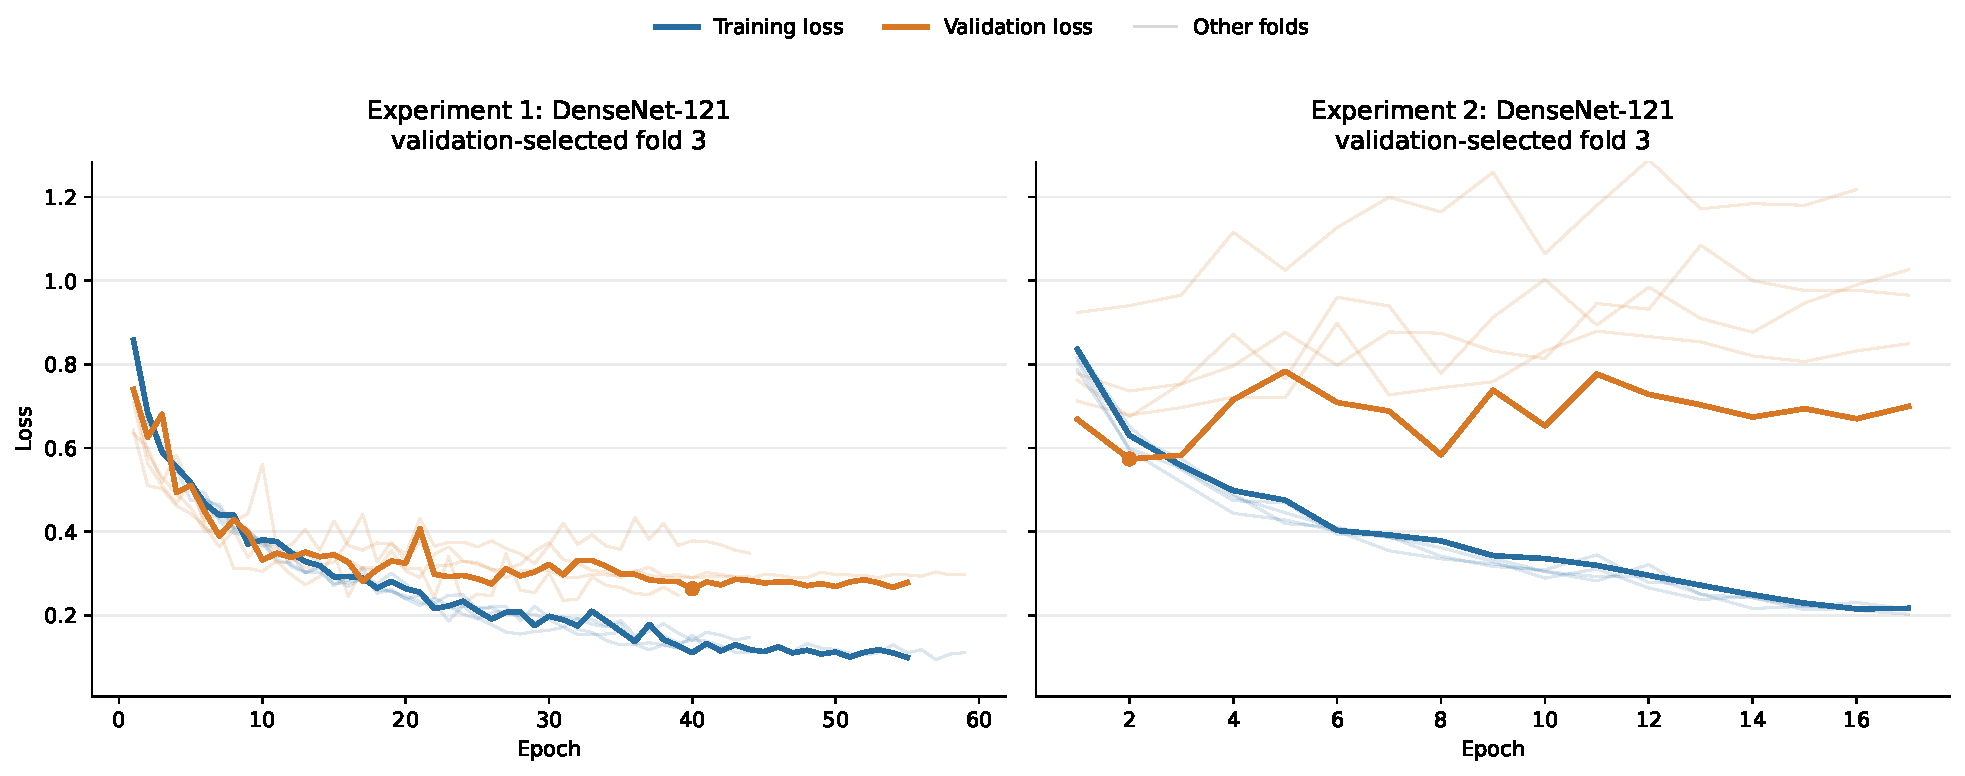
\includegraphics[width=\textwidth]{fig_train_validation_loss.pdf}
\caption{Training and validation loss for the best-performing architecture in each experiment. Lighter lines show all five folds, while darker lines show the fold selected using validation balanced accuracy. The point marks the minimum validation loss of the selected fold.}
\label{fig:train-validation-loss}
\end{figure*}

\begin{figure*}[t]
\centering
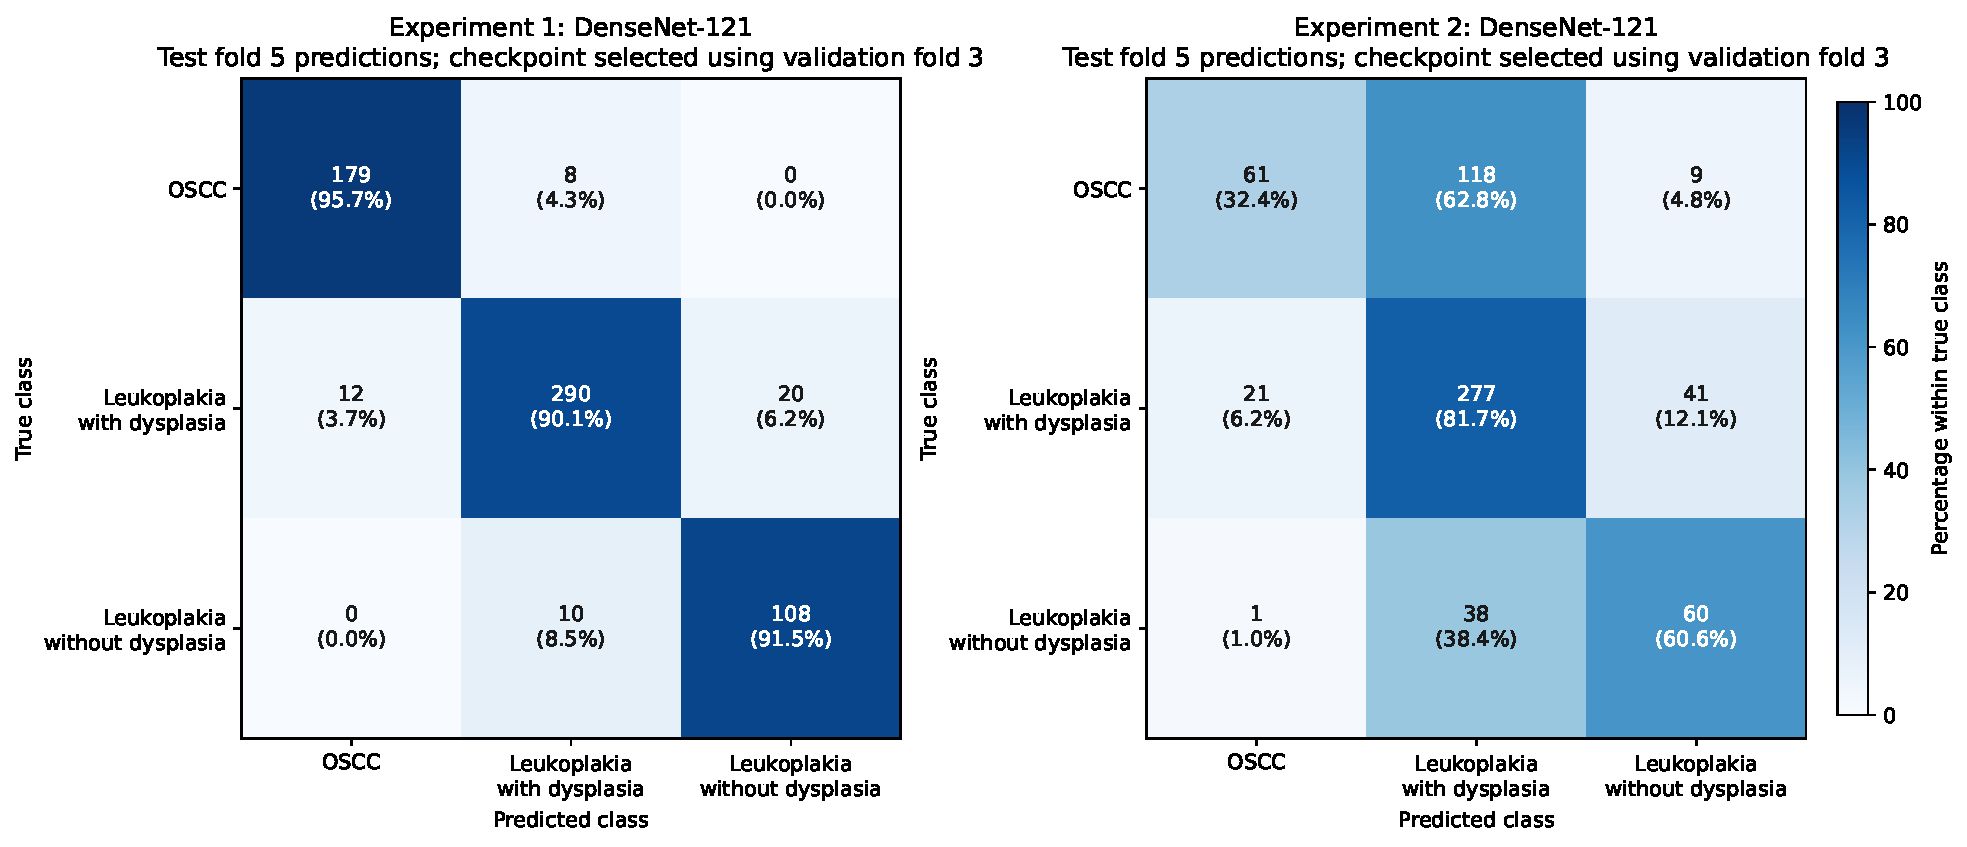
\includegraphics[width=\textwidth]{fig_confusion_matrices.pdf}
\caption{Held-out confusion matrices for the validation-selected DenseNet-121 checkpoint in each experiment. Cells report counts and percentages within each true class.}
\label{fig:confusion-matrices}
\end{figure*}
